\documentclass[conference]{IEEEtran}
%\IEEEoverridecommandlockouts
% The preceding line is only needed to identify funding in the first footnote. If that is unneeded, please comment it out.
\usepackage[spanish]{babel}
\usepackage[utf8]{inputenc}
\usepackage{cite}
\usepackage{amsmath, amsthm,amssymb,amsfonts}
\usepackage{algorithmic}
\usepackage{graphicx}
\usepackage{textcomp}
\usepackage{xcolor}
\def\BibTeX{{\rm B\kern-.05em{\sc i\kern-.025em b}\kern-.08em
    T\kern-.1667em\lower.7ex\hbox{E}\kern-.125emX}}

% Definición del entorno 'definition'
\newtheorem{definition}{Definición}

\begin{document}

\title{Control Robusto Multivaluado: La Importancia de la Monotonía en Problemas Bien Definidos\\
	% {\footnotesize \textsuperscript{*}Note: Sub-titles are not captured in Xplore and
	% should not be used}
	% \thanks{Identify applicable funding agency here. If none, delete this.}
}

\author{
	\IEEEauthorblockN{José Alejandro León Sánchez}
	\IEEEauthorblockA{\textit{Posgrado de Ingeniería} \\
		\textit{UNAM}\\
		CDMX, Mexico}
	\and
	\IEEEauthorblockN{Fernando Castaños Luna}
	\IEEEauthorblockA{\textit{CINVESTAV} \\
		\textit{IPN}\\
		CDMX, Mexico}
}

\maketitle

\begin{abstract}
	Este documento es un resumen de la segunda ponencia del Seminario de Investigación de la Maestría en Ingeniería Eléctrica (Especialización en Control) del programa de Posgrado en Ingeniería de la UNAM, presentada por el Dr. Fernando Castaños. En esta presentación se abordó el concepto de funciones multivaluadas, introducidas de manera intuitiva a través de ejemplos prácticos como el comportamiento de diodos y restricciones mecánicas unilaterales. A partir de estos ejemplos, se discutieron las inclusiones resultantes, también conocidas como ecuaciones generalizadas, y se extendió el análisis hacia las inclusiones diferenciales, con el fin de introducir el concepto de monotonía y su papel en garantizar que las ecuaciones generalizadas estén bien planteadas.

	Posteriormente, se presentaron esquemas de control basados en leyes de control multivaluadas, como los modos deslizantes, destacando su relevancia en sistemas robustos. Para concluir, se exploraron técnicas de discretización de estos controladores, subrayando que la discretización implícita de Euler ofrece mejores resultados comparada con la versión explícita, en términos de estabilidad y precisión.
\end{abstract}

\begin{IEEEkeywords}
	Control robusto, Funciones multivaluadas, Inclusiones diferenciales, Monotonía, Modos deslizantes, Discretización implícita, Discretización explícita, Control multivaluado
\end{IEEEkeywords}


\section{Introducción}
En el campo del control de sistemas dinámicos, la robustez frente a perturbaciones externas e incertidumbres en los modelos es un desafío fundamental. Los controladores robustos deben ser capaces de operar eficazmente en entornos no ideales, donde las características del sistema pueden variar o no ser completamente conocidas. En este contexto, las leyes de control multivaluadas ofrecen una herramienta poderosa para enfrentar tales desafíos, aprovechando su capacidad de manejar soluciones no únicas y, con ello, proporcionar una mayor robustez.

La presente ponencia introduce el concepto de leyes de control multivaluadas y su aplicación en sistemas físicos con componentes que exhiben comportamientos no lineales y multivaluados, como diodos y restricciones mecánicas unilaterales. Se exploran las ventajas de este enfoque para mejorar la estabilidad y robustez de sistemas sujetos a incertidumbres. Además, se aborda la discretización de estas leyes de control, una etapa esencial para su implementación en dispositivos digitales, como microprocesadores y microcontroladores.

\section{Introducción intuitiva a las funciones multivaluadas}

El concepto de funciones multivaluadas fue introducido mediante el ejemplo de un diodo ideal. Este componente permite el paso de corriente cuando el voltaje es positivo y bloquea la corriente en sentido contrario o cuando el voltaje es cero. Este comportamiento puede representarse a través de la relación entre corriente \( i_d \) y voltaje \( v_d \) de manera multivaluada:

\begin{equation}
	i_d \in \begin{cases}
		\emptyset    & \text{si } v_d < 0 \\
		\mathbb{R}_+ & \text{si } v_d = 0 \\
		\{0\}        & \text{si } v_d > 0
	\end{cases}
\end{equation}

Alternativamente, se puede describir mediante:

\begin{equation}
	i_d \geq 0, \quad v_d \geq 0, \quad i_d \cdot v_d = 0
\end{equation}

Finalmente, el comportamiento del diodo también se expresa mediante el subdiferencial:

\begin{equation}
	i_d \in -\partial \Psi_{\mathbb{R}_+}(v_d)
\end{equation}

Este ejemplo ilustra cómo las funciones multivaluadas capturan relaciones no únicas en sistemas físicos, como ocurre en los diodos y otros elementos no lineales. Sin embargo, al tener en cuenta restricciones como una resistencia conectada, vemos que se seleccionará un valor único de corriente, esta propiedad es útil en el contexto de control robusto (figura \ref{fig:caracteristica}).

\begin{figure}[h]
	\centering
	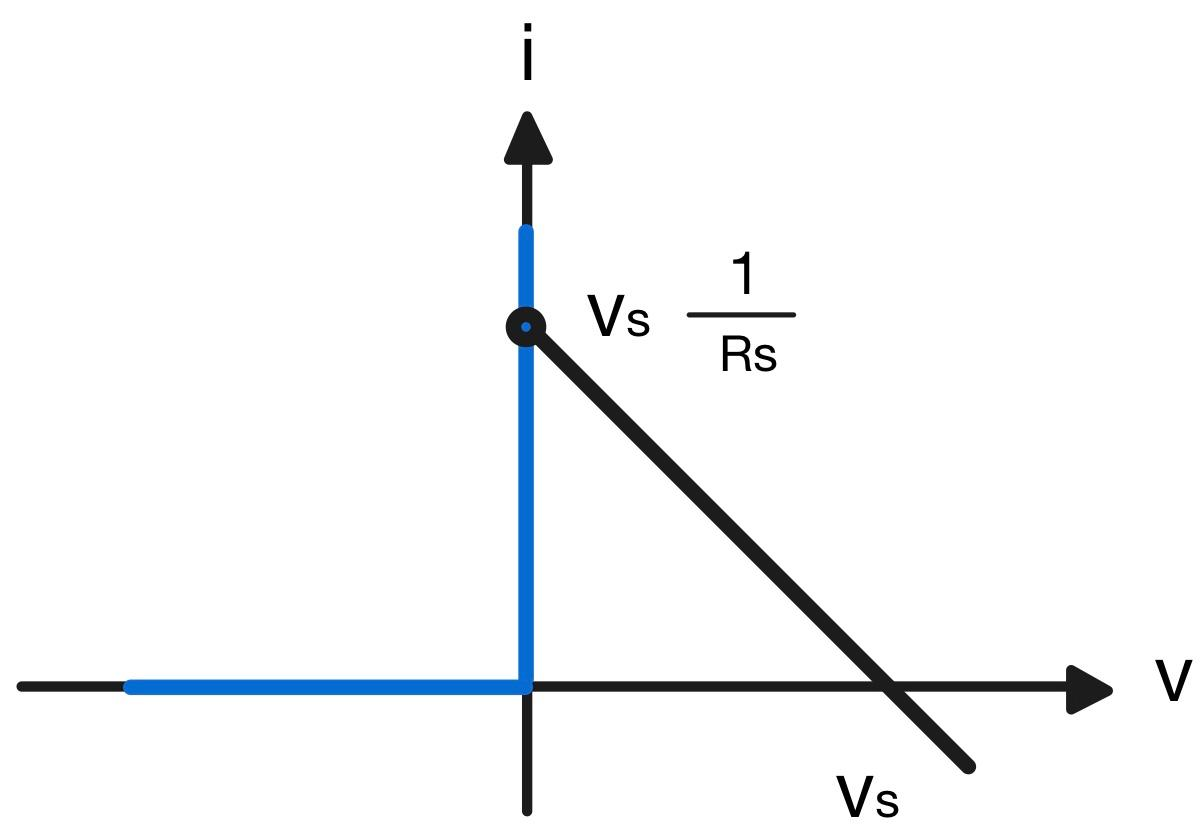
\includegraphics[width=0.5\textwidth]{v_vs_i.jpeg}
	\caption{Característica voltaje-corriente un circuito simple con diodo y resistencia}
	\label{fig:caracteristica}
\end{figure}


\section{Monotonía y problemas bien definidos}

En la presentación se abordó la importancia de la \textit{monotonía} en los sistemas multivaluados y cómo esta propiedad garantiza la existencia y unicidad de soluciones en problemas de control robusto. Un operador multivaluado \( M: \mathbb{R}^n \rightrightarrows \mathbb{R}^n \) se dice que es monótono si, para cada \( z \in M(x) \) y \( \xi \in M(\xi) \), se cumple la siguiente condición:

\begin{equation}
	\langle z - \xi, x - \xi \rangle \geq 0, \quad \forall \, \xi \in M(\xi)
\end{equation}

Esta propiedad es particularmente relevante en el diseño de controladores robustos, ya que un operador que es \textit{máximamente monótono} asegura que no existe otro operador monótono que contenga a \( M(x) \). La \textit{monotonía máxima} garantiza que la inclusión diferencial asociada tiene una solución única, lo que es fundamental para que el problema esté bien definido.

Un ejemplo práctico de este tipo de fenómenos es el modelado de sistemas con fricción seca. La relación entre la fuerza de fricción y la velocidad se puede representar mediante una inclusión diferencial:

\begin{equation}
	m \dot{v}(t) \in \mu F_N \, \text{Sgn}(v(t)) + F_e(t)
\end{equation}

Este tipo de ecuaciones son típicas de sistemas físicos con elementos no lineales y multivaluados, como los diodos y la fricción, y demuestran cómo la monotonía permite abordar problemas de estabilidad y unicidad de soluciones. En el contexto del control, asegurar la \textit{monotonía máxima} es clave para que las soluciones converjan a un valor deseado bajo condiciones de perturbación e incertidumbre.


\section{Control multivaluado}

El control multivaluado se aplica en sistemas donde la relación entre las variables no es única, como ocurre en el control por modos deslizantes. El diseño de estos controladores se basa en dos pasos fundamentales. Primero, se define una salida virtual \( \sigma(x) \), de tal manera que si \( \sigma(x(t)) = 0 \), entonces \( x(t) \) converge a un valor deseado \( x^* \):

\begin{equation}
	\sigma(x(t)) = 0 \quad \Rightarrow \quad \lim_{t \to \infty} x(t) = x^*
\end{equation}

En segundo lugar, se implementa una ley de control multivaluada que asegura que la dinámica del sistema converja a la superficie de deslizamiento. Por ejemplo:

\begin{equation}
	u(t) \in -\gamma \, \text{Sgn}(\sigma(t))
\end{equation}

Este tipo de control asegura robustez ante perturbaciones externas \( d(t) \), manteniendo el sistema dentro de una banda de error controlada.

\section{Implementación en tiempo discreto}

Para la implementación en tiempo discreto de controladores multivaluados, se utiliza típicamente la discretización implícita de Euler, la cual preserva las propiedades de estabilidad del sistema. El sistema discreto se puede aproximar mediante la ecuación en diferencias:

\begin{equation}
	\sigma_{k+1} = \sigma_k + h \, u_k
\end{equation}

Donde \( u_k \) se determina resolviendo la inclusión multivaluada en cada paso de tiempo. A diferencia de la discretización explícita, el método implícito garantiza que el sistema siga siendo robusto ante perturbaciones y preserve la estabilidad global del controlador, haciéndolo adecuado para su implementación en microcontroladores con tiempos de muestreo relativamente bajos.


\section*{Conclusiones}
\section{Conclusiones}

El control multivaluado se presenta como una herramienta poderosa para abordar sistemas con relaciones no únicas entre variables, como ocurre en el control por modos deslizantes. Este enfoque permite diseñar controladores robustos ante perturbaciones e incertidumbres del sistema, garantizando la convergencia a la superficie de deslizamiento y manteniendo un rendimiento estable.

La implementación en tiempo discreto de estos controladores, a través de la discretización implícita de Euler, permite preservar las propiedades de estabilidad y robustez, haciendo viable su uso en sistemas embebidos con tiempos de muestreo limitados. Esta discretización es crucial para asegurar que las características del controlador multivaluado se mantengan intactas durante la discretización.

\begin{thebibliography}{00}
	\bibitem{operadores_monotonos_2018}
	“Operadores monótonos”, Proyecciones (Antofagasta, On line), vol. 2, no. 6, pp. 67–102, Mar. 2018, doi: 10.22199/S07160917.1983.0006.00004.

	\bibitem{castanos_2022}
	F. Castaños, "Multi-valued control of port-Hamiltonian systems", Revista Iberoamericana de Automática e Informática Industrial, vol. 19, pp. 419–429, 2022, doi: 10.4995/riai.2022/16814.

\end{thebibliography}

\end{document}
